\let\negmedspace\undefined
\let\negthickspace\undefined
\documentclass[journal]{IEEEtran}
\usepackage[a5paper, margin=10mm, onecolumn]{geometry}
%\usepackage{lmodern} % Ensure lmodern is loaded for pdflatex
\usepackage{tfrupee} % Include tfrupee package

\setlength{\headheight}{1cm} % Set the height of the header box
\setlength{\headsep}{0mm}     % Set the distance between the header box and the top of the text

\usepackage{gvv-book}
\usepackage{gvv}
\usepackage{cite}
\usepackage{amsmath,amssymb,amsfonts,amsthm}
\usepackage{algorithmic}
\usepackage{graphicx}
\usepackage{textcomp}
\usepackage{xcolor}
\usepackage{txfonts}
\usepackage{listings}
\usepackage{enumitem}
\usepackage{mathtools}
\usepackage{gensymb}
\usepackage{comment}
\usepackage[breaklinks=true]{hyperref}
\usepackage{tkz-euclide} 
\usepackage{listings}
% \usepackage{gvv}                                        
\def\inputGnumericTable{}                                 
\usepackage[latin1]{inputenc}                                
\usepackage{color}                                            
\usepackage{array}                                            
\usepackage{longtable}                                       
\usepackage{calc}                                             
\usepackage{multirow}                                         
\usepackage{hhline}                                           
\usepackage{ifthen}                                           
\usepackage{lscape}
\begin{document}

\bibliographystyle{IEEEtran}
\vspace{3cm}

\title{1-1.7-8}
\author{EE24BTECH11058 - P.Shiny Diavajna}
% \maketitle
% \newpage
% \bigskip
{\let\newpage\relax\maketitle}

\renewcommand{\thefigure}{\theenumi}
\renewcommand{\thetable}{\theenumi}
\setlength{\intextsep}{10pt} % Space between text and floats


\numberwithin{equation}{enumi}
\numberwithin{figure}{enumi}
\renewcommand{\thetable}{\theenumi}


\textbf{Question}:Using vectors,prove that the points $\brak{2,-1,3}$,$\brak{3,-5,1}$ and $\brak{-1,11,9}$ are collinear. \\

\solution 
\begin{table}[h!]    
  \centering
  \begin{tabular}[12pt]{ |c| c|}
    \hline
    \textbf{Variable} & \textbf{Description}\\ 
    \hline
	$\myvec{2&-1&3}$ & Point $\vec{A}$\\
    \hline 
	$\myvec{3&-5&1}$ & Point $\vec{B}$\\
    \hline
	$\myvec{-1&11&9}$ & Point $\vec{C}$\\
    \hline   
\end{tabular}

  \caption{Variables Used}
  \label{tab1-1.7-8.1}
\end{table}

  \begin{align*}
	\myvec{B-A & C-A}^\top =\myvec{1 & -4 & -2 \\-3 & 12 &6}\\
	\xrightarrow{R_2=R_2+3R_1} \myvec{1 & -4 &-2\\ 0 & 0 &0}\\ 
  \end{align*} 

  \begin{align*}
	\text{rank = number of non-zero rows}\\
	\text{i.e. rank =1}\\
  \end{align*}
	

therefore,\\ 
\begin{align*}	
	\vec{A}, \vec{B} , \vec{C} \text{ are collinear.}\\
\end{align*}



  \begin{figure}[h!]
   \centering
   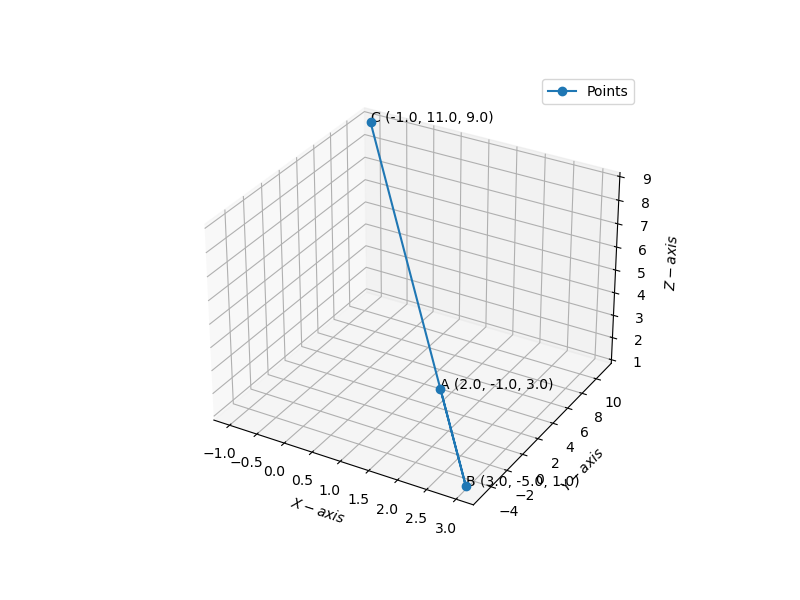
\includegraphics[width=0.7\linewidth]{/home/shiny/Desktop/mt/assignment4/figs/Figure_3.png}
   \caption{Plot of points A,B and C}
  \end{figure}
\end{document}  
